\clearpage
\section{Atmospheric parameters before and after the BIC scan}
\label{app:atmo_pre_post_bic}

This appendix shows the per-star comparison of the atmospheric parameters
between the full-magnetic run and the BIC-selected run, discussed in
Sect.~\ref{sec:results_bic}. Figures~\ref{fig:pre_post_bic_teff}--\ref{fig:pre_post_bic_mh}
present $T_\mathrm{eff}$, $\log g$, and $[\mathrm{M/H}]$ in turn; both runs use the
same region-filtered line lists, and the lower panel of each figure gives the
per-star difference (full minus BIC-selected).

\begin{figure*}[!h]
    \centering
    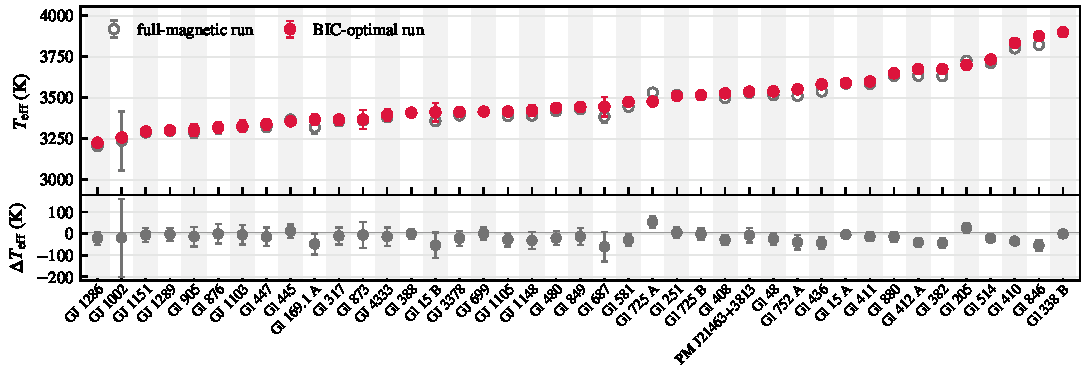
\includegraphics[width=.98\linewidth]{figures/teff_pre_and_post_bic_scan.pdf}
    \caption{Retrieved $T_\mathrm{eff}$ from the full-magnetic run (open grey) and the BIC-selected run (filled red), ordered by the BIC-selected $T_\mathrm{eff}$. The lower panel shows the per-star difference (full minus BIC-selected). The dashed line marks the median. Median residual $+2.3$~K.}
    \label{fig:pre_post_bic_teff}
\end{figure*}

\begin{figure*}[!h]
    \centering
    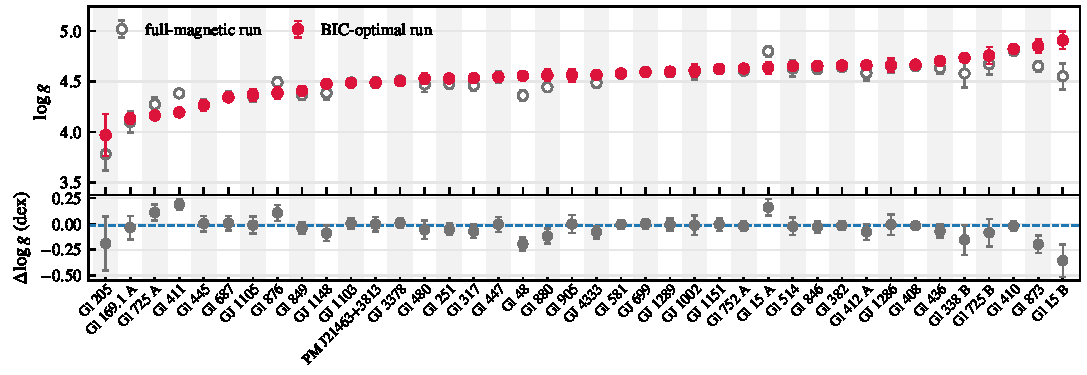
\includegraphics[width=.98\linewidth]{figures/logg_pre_and_post_bic_scan.pdf}
    \caption{As Fig.~\ref{fig:pre_post_bic_teff}, but for $\log g$. Median residual $-0.02$~dex.}
    \label{fig:pre_post_bic_logg}
\end{figure*}

\begin{figure*}[!h]
    \centering
    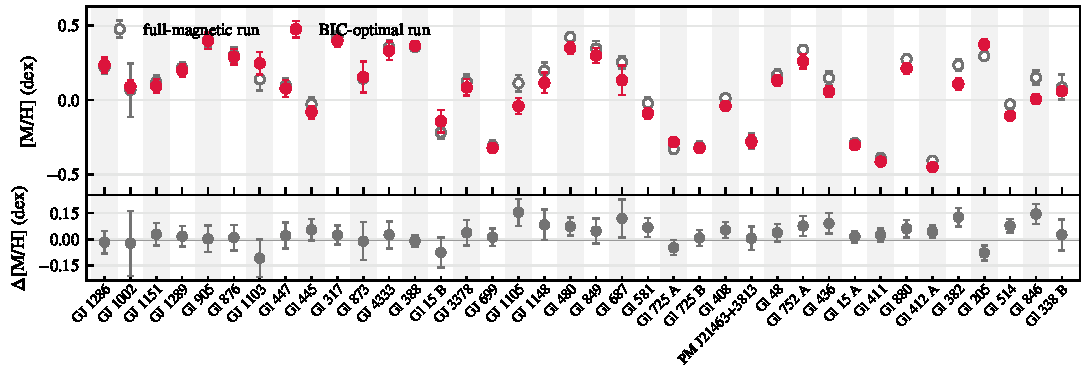
\includegraphics[width=.98\linewidth]{figures/mh_pre_and_post_bic_scan.pdf}
    \caption{As Fig.~\ref{fig:pre_post_bic_teff}, but for $[\mathrm{M/H}]$. Median residual $-0.002$~dex.}
    \label{fig:pre_post_bic_mh}
\end{figure*}
